%----------------------------------------------------------------------------------------
%	PACKAGES AND OTHER DOCUMENT CONFIGURATIONS
%----------------------------------------------------------------------------------------

\documentclass[
	a4paper, % Paper size, use either a4paper or letterpaper
	10pt, % Default font size, can also use 11pt or 12pt, although this is not recommended
	unnumberedsections, % Comment to enable section numbering
	twoside, % Two side traditional mode where headers and footers change between odd and even pages, comment this option to make them fixed
]{LTJournalArticle}

\usepackage{array}
\usepackage{pgfplots}
\usepackage{verbatim}
\usepackage{amsmath}
\usepackage{mathtools}

\addbibresource{sample.bib} % BibLaTeX bibliography file

\runninghead{Software Engineering Skills Analysis} % A shortened article title to appear in the running head, leave this command empty for no running head

\footertext{\textit{Tyler Mong, CSCI-3327-001 Project 2} (2025)} % Text to appear in the footer, leave this command empty for no footer text

\setcounter{page}{1} % The page number of the first page, set this to a higher number if the article is to be part of an issue or larger work

%----------------------------------------------------------------------------------------
%	TITLE SECTION
%----------------------------------------------------------------------------------------

\title{Applying Statistical Methods to Analyze Software Engineering Skills: A Data-Driven Approach to Maximizing Internship Success} % Article title, use manual lines breaks (\\) to beautify the layout

% Authors are listed in a comma-separated list with superscript numbers indicating affiliations
% \thanks{} is used for any text that should be placed in a footnote on the first page, such as the corresponding author's email, journal acceptance dates, a copyright/license notice, keywords, etc
\author{%
	Tyler Mong\textsuperscript{1}
}

% Affiliations are output in the \date{} command
\date{\footnotesize\textsuperscript{\textbf{1}}School of Business - Computer Science, Stockton University}

% Full-width abstract
\renewcommand{\maketitlehookd}{%
	\begin{abstract}
		\noindent This paper analyzes 199 software engineering internship listings to identify the most in-demand technical skills. Python, C++, and Java were the most frequently mentioned skills, appearing in 38\%, 24\%, and 21\% of listings, respectively. The data follows a right-skewed distribution, indicating that a small number of skills are dominant. Furthermore, these dominant skills are typically widely adopted and stable technologies, rather than newer, trendier ones. This analysis has several limitations, particularly the small sample size, and future improvements could include increasing the sample size and integrating a machine learning model for more advanced analysis.
	\end{abstract}
}

%----------------------------------------------------------------------------------------

\begin{document}

\maketitle % Output the title section

%----------------------------------------------------------------------------------------
%	ARTICLE CONTENTS
%----------------------------------------------------------------------------------------

\section{Introduction}

The software engineering job market continues to be in a highly competitive state, especially for those trying to break into tech by applying to new graduate and internship roles. Companies are increasingly seeking interns who possess strong technical abilities and can demonstrate their skills through live technical interviews. Additionally, with waves of layoffs and the rapid rise of artificial intelligence, the average computer science student is facing increased pressure to stand out in a crowded field. As such, it is essential for students to understand which skills are most in demand in order to remain competitive when applying to internship roles.

This study explores the skills required in software engineering internship positions by analyzing approximately 200 internship listings scraped from various job boards. The listings represent a wide range of companies, from big tech companies to smaller startups, providing a broad perspective on current industry expectations. The primary objective of this analysis is to identify the most in-demand technical skills across software engineering internships.

Through this research, statistical methods taught throughout the CSCI-3327 Probability and Applied Statistics course at Stockton University are applied to a series of sample problems, and the results are analyzed. 

%------------------------------------------------

\section{Methods}

\subsection{Data Collection}

Internship listings were scraped using a Java-based script with the \textit{jsoup}\footnote{\textit{jsoup}: the Java HTML parser, built for HTML editing, cleaning, scraping, and XSS safety. Available at: \url{https://jsoup.org/}.} library, which is built to parse webpage data. The data collection process was carried out as follows:

\begin{enumerate}
    \item \textbf{Link Scraping}: Internship listing links were scraped from two GitHub repositories: Summer 2025 Tech Internships by Pitt CSC \& Simplify, and Summer 2025 Tech Internships by Vansh \& Ouckah. These repositories provided collections of links to internship listings hosted on various platforms.
    \item \textbf{Duplicate Link Filtering}: Duplicate links were removed from the dataset to ensure each internship listing was only included once.
    \item \textbf{Platform Link Filtering}: The remaining links were further filtered to include only those hosted on the Workday, Greenhouse, and Lever job platforms. Although the dataset spans 2,173 links across 436 different job boards, the three aforementioned platforms together account for approximately 28\% of all links, despite representing only 0.69\% of the total number of job boards.
    \item \textbf{Data Scraping}: After filtering, the remaining internship listings were scraped for key information, including company name, job title, location, skills, and listing URL. Skills were extracted by identifying technical keywords\footnote{A full list of keywords can be found in: \url{src/main/java/dev/tylermong/jobanalyzer/util/SkillKeywords.java}}, such as programming languages, frameworks, and tools, mentioned in the job description. Skills were standardized to be case-insensitive to group together the same skills with different capitalizations.
\end{enumerate}
\subsection{Statistical Analysis}
The processed data was analyzed using a Java-based approach, where each skill keyword was stored as a key in a map, with the corresponding frequency of occurrences as the value. These key-value pairs were then written to a file for easy viewing. This simple frequency analysis lays the foundation for potential further statistical exploration, such as identifying trends or comparing skill frequencies across different internship listings.


%------------------------------------------------

\section{Results}

\subsection{Skill Frequency Distribution}

\begin{table}[h]
    \centering
    \begin{tabular}{|>{\centering\arraybackslash}p{3cm}|>{\centering\arraybackslash}p{1cm}|>{\centering\arraybackslash}p{1cm}|}
        \cline{1-3}
        \textbf{Skill} & \textbf{\#} & \textbf{\%} \\ \cline{1-3}
        Python & 75 & 38\% \\ \cline{1-3}
        C++ & 47 & 24\% \\ \cline{1-3}
        Java & 41 & 21\% \\ \cline{1-3}
        Algorithms & 37 & 19\% \\ \cline{1-3}
        AI & 34 & 17\% \\ \cline{1-3}
        Agile & 26 & 13\% \\ \cline{1-3}
        JavaScript & 25 & 13\% \\ \cline{1-3}
        Linux & 22 & 11\% \\ \cline{1-3}
        C & 21 & 11\% \\ \cline{1-3}
        SQL & 19 & 10\% \\ \cline{1-3}
    \end{tabular}
    \caption{Top 10 most frequent skills across 199 internship listings.}
    \label{tab:skills_frequency}
\end{table}

As shown in the Table \ref{tab:skills_frequency}, Python leads as the most popular skill, appearing in 38\% of internship listings, followed by C++ and Java at 24\% and 21\% respectively. The median skill frequency occurrence is 1\%, with the mean being 2.9\%. This disparity indicates a heavily right-skewed distribution, where a small set of highly demanded skills dominates the market, and the majority of skills form a long tail of lower demand.

\vspace{5cm}
\subsection{Problems and Solutions Using Scraped Data}

% [START] Chapter 1, Problem 1
\subsubsection{1.1}
\textbf{Are some skills more common than others? Given below are the frequency of skills for 20 randomly selected software engineering skills:
\begin{table}[h!]
    \centering
    \begin{tabular}{ccccc}
        2 & 6 & 4 & 7 & 18 \\
        1 & 17 & 3 & 75 & 34 \\
        10 & 37 & 16 & 5 & 21 \\
        9 & 25 & 8 & 41 & 14 \\
    \end{tabular}
    \caption{20 randomly selected skill occurrences from 199 internship listings.}
    \label{tab:table_p1.1}
\end{table}
\\ a. Construct a relative frequency histogram for this data.
}

    % Histogram
    \begin{figure}[h!]
        \centering
        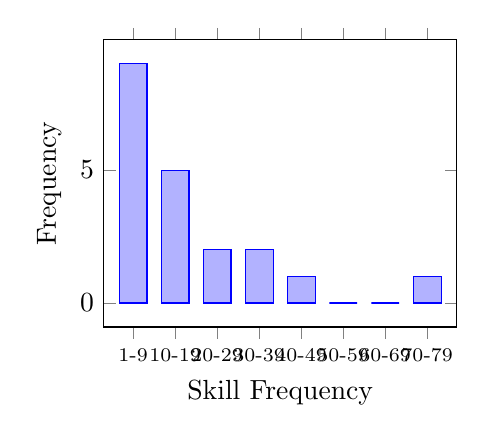
\begin{tikzpicture}
            \begin{axis}[
                ybar,
                symbolic x coords={1-9, 10-19, 20-29, 30-39, 40-49, 50-59, 60-69, 70-79},
                xtick=data,
                ylabel={Frequency},
                xlabel={Skill Frequency},
                xticklabel style={font=\scriptsize},
                width=0.5\textwidth
            ]
            \addplot coordinates {(1-9, 9) (10-19, 5) (20-29, 2) (30-39, 2) (40-49, 1) (50-59, 0) (60-69, 0) (70-79, 1)};
            \end{axis}
        \end{tikzpicture}
        \caption{Relative Frequency Histogram of Skill Occurrences}
        \label{fig:histogram_p1.1}
    \end{figure}
% [END] Chapter 1, Problem 1

% [START] Chapter 2, Problem 1
\subsubsection{2.1}
\textbf{A company is reviewing four internship applications with each applicant highlighting a different primary skill (Python, C++, Java, AI). The company random selects two applicants to interview.} \\
\\ \textbf{a. List all possible pairs of applicants selected.}
\begin{equation*}
    \begin{aligned}
        \text{\{(Python, C++), (Python, Java), (Python, AI),} \\
        \text{(C++, Java), (C++, AI), (Java, AI)\}}
    \end{aligned}
\end{equation*}

\textbf{b. Assign reasonable probabilities to each pair.}
\begin{equation*}
    \begin{aligned}
        \text{All pairs have an equal probability of } \frac{1}{6} \text{.}
    \end{aligned}
\end{equation*}

\textbf{c. Find the probability that the applicant with Java as their primary skill is selected for an interview.} \\
\begin{equation*}
    \begin{aligned}
        P(\text{Java selected}) = \frac{3}{6} = \frac{1}{2}
    \end{aligned}
\end{equation*}
% [END] Chapter 2, Problem 1

% [START] Chapter 2, Problem 2
\subsubsection{2.2}
\textbf{An intern needs to attend two different training sessions on separate days: one about programming languages (6 options) and one about software engineering methodologies (7 options). How many different two-session training combinations can the intern choose?}

\begin{equation*}
    \begin{aligned}
        6 \times 7 = 42
    \end{aligned}
\end{equation*}
% [END] Chapter 2, Problem 2
\vspace*{1pt}\noindent
% [START] Chapter 2, Problem 3
\subsubsection{2.3}
\textbf{An internship program is reviewing applicants for a software engineering position. There are 52 applicants, each with one primary skill: Python, C++, Java, or AI. The skills are evenly divided, meaning there are 13 applicants for each skill.} \\

\textbf{a. If the first two selected applicants both specialize in Python, what is the probability that the next three selected applicants will also specialize in Python?} \\
\begin{equation*}
    \begin{aligned}
        P(\text{3 more Python selected}) &= \frac{11}{50} \times \frac{10}{49} \times \frac{9}{48} \\
        &= 0.00841 = 0.84\%
    \end{aligned}
\end{equation*}
\vspace{2pt}

\textbf{b. If the first three selected applicants all specialize in Python, what is the probability that the next two selected applicants will also specialize in Python?} \\
\begin{equation*}
    \begin{aligned}
        P(\text{2 more Python selected}) &= \frac{10}{49} \times \frac{9}{48} \\
        &= 0.03826 = 3.82\%
    \end{aligned}
\end{equation*}
\vspace{2pt}

\textbf{c. If the first four selected applicants all specialize in Python, what is the probability that the next selected applicant will also specialize in Python?} \\
\begin{equation*}
    \begin{aligned}
        P(\text{1 more Python selected}) &= \frac{9}{48} \\ 
        & = 0.1875 = 18.75\%
    \end{aligned}
\end{equation*}
% [END] Chapter 2, Problem 3
\vspace*{1pt}\noindent
% [START] Chapter 2, Problem 4
\subsubsection{2.4}
\textbf{Two events, $A$ (an applicant knowing Python) and $B$ (an applicant knowing C++), are such that $P(A) = .2$, $P(B) = .3$, and $P(A \cup B) = .4$. Find the following:} \\

\textbf{a. $P(A \cap B)$}
\begin{equation*}
    \begin{aligned}
        P(A \cap B) &= P(A) + P(B) - P(A \cup B) \\
        P(A \cap B) &= 0.2 + 0.3 - 0.4 = 0.1 \\
    \end{aligned}
\end{equation*}

\textbf{b. $P(\overline A \cup \overline B)$} \\
\begin{equation*}
    \begin{aligned}
        P(\overline A \cup \overline B) &= 1 - P(A \cap B) \\
        P(\overline A \cup \overline B) &= 1 - 0.1 = 0.9 \\
    \end{aligned}
\end{equation*}

\textbf{c. $P(\overline A \cap \overline B)$}
\begin{equation*}
    \begin{aligned}
        P(\overline A \cap \overline B) &= 1 - P(A \cup B) \\
        P(\overline A \cap \overline B) &= 1 - 0.4 = 0.6
    \end{aligned}
\end{equation*}


\textbf{d. $P(\overline A | B)$} \\
\begin{equation*}
    \begin{aligned}
        P(\overline A | B) &= \frac{P(\overline{A}\cap B)}{P(B)} \\
        P(\overline A \cap B) &= P(B) - P(A \cap B) = 0.3 - 0.1 = 0.2 \\
        P(\overline A | B) &= \frac{0.2}{0.3} = \frac{2}{3}
    \end{aligned}
\end{equation*}
% [END] Chapter 2, Problem 4
\vspace*{1pt}\noindent
% [START] Chapter 2, Problem 5
\subsubsection{2.5}
\textbf{Five interns are randomly selected from 52 total interns, who are divided evenly among 4 different teams, based on their preferred language (frontend, backend, data science, and AI/ML). What is the probability that all five selected new hires are from the same team?} \\
\begin{equation*}
    \begin{aligned}
        \binom{52}{5} &= 2,598,960 \text{ total ways}\\ 
        \binom{13}{5} &= 1287 \times 4 = 5148 \text{ favorable ways} \\
        P(\text{All same team)} &= \frac{5148}{2,598,960} = 0.00198 = 0.198\%
    \end{aligned}
\end{equation*}
% [END] Chapter 2, Problem 5
\vspace*{1pt}\noindent
% [START] Chapter 3, Problem 1
\subsubsection{3.1}
\textbf{An application randomly maps three input field labels to three corresponding data fields. If the labels are assigned randomly, let $Y$ be the number of labels correctly matched to their intended fields. Determine the probability distribution of $Y$.} \\
\begin{equation*}
    \begin{aligned}
        \text{Correct order: (1, 2, 3)} \\
        1, 2, 3: 3 \text{ correct} \\
        1, 3, 2: 1 \text{ correct} \\
        2, 1, 3: 1 \text{ correct} \\
        2, 3, 1: 0 \text{ correct} \\
        3, 1, 2: 0 \text{ correct} \\
        3, 2, 1: 1 \text{ correct} \\
    \end{aligned}
\end{equation*}
\begin{equation*}
    \begin{aligned}
        P(Y = 0) = \frac{2}{6} &= \frac{1}{3} \\
        P(Y = 1) = \frac{3}{6} &= \frac{1}{2} \\
        P(Y = 2) &= 0 \\
        P(Y = 3) &= \frac{1}{6} \\
    \end{aligned}
\end{equation*}
% [END] Chapter 3, Problem 1
\vspace*{50pt}\noindent
% [START] Chapter 3, Problem 2
\subsubsection{3.2}
\textbf{A fault-tolerant distributed software system includes four redundant service modules that perform the same task. Each module has a 20\% chance of crashing within 1000 hours. The system is designed to remain operational as long as at least two of the four modules are running. Assume each module fails independently.} \\

\textbf{a. What is the probability that exactly two out of the four modules survive past 1000 hours?} \\
\begin{equation*}
    \begin{aligned}
        P(Y = 2) &= \binom{4}{2} \cdot (0.8)^2 \cdot (0.2)^2 \\ 
        &= 6 \cdot 0.64 \cdot 0.04 = 0.1536 \\
    \end{aligned}
\end{equation*} \\

\textbf{b. What is the probability that the system as a whole continues functioning beyond 1000 hours?} \\
\begin{equation*}
    \begin{aligned}
        P(\text{system works}) &= P(Y \ge 2) \\ 
        P(Y \ge 2) &= 1 - P(Y = 0) - P(Y = 1) \\
        P(Y = 0) &= \binom{4}{0} \cdot (0.8)^0 \cdot (0.2)^4 = 0.0016 \\ 
        P(Y = 1) &= \binom{4}{1} \cdot (0.8)^1 \cdot (0.2)^3 = 0.0256 \\
        P(Y \ge 2) &= 1 - 0.0016 - 0.0256 = 0.9728 \\
    \end{aligned}
\end{equation*}
% [END] Chapter 3, Problem 2
\vspace*{1pt}\noindent
% [START] Chapter 3, Problem 3
\subsubsection{3.3}
\textbf{Suppose that 30\% of software engineering internship applicants report proficiency in Python. Applicants are interviewed one at a time and selected at random from the pool. What is the probability that the first applicant with Python experience is found on the fifth interview?} \\
\begin{equation*}
    \begin{aligned}
        P(Y = 5) &= q^{y - 1} \cdot p \\
        &= (0.70)^4 \cdot 0.30 \\
        &= 0.07203
    \end{aligned}
\end{equation*}
% [END] Chapter 3, Problem 3
\vspace*{1pt}\noindent
% [START] Chapter 3, Problem 4
\subsubsection{3.4}
\textbf{10\% of applicants in an applicant pool lack essential SQL skills. Applicants are interviewed one by one and randomly selected. What is the probability that the first candidate with strong SQL skills will be found in the second interview?}
\begin{equation*}
    \begin{aligned}
        P(Y = 2) &= (0.1)^1 \cdot (0.9) \\
        &= 0.09
    \end{aligned}
\end{equation*}
% [END] Chapter 3, Problem 4
\vspace*{100pt}\noindent
% [START] Chapter 3, Problem 5
\subsubsection{3.5}
\textbf{An applicant pool contains 10 applicants, of which 5 list Python as a skill, 2 list C++, and 3 list Java. If 3 applicants are selected one at a time without replacement, what is the probability that all three selected applicants list Python on their resume?}
\begin{equation*}
    \begin{aligned}
        P(Y = 5) &= \frac{\binom{5}{3} \binom{5}{0}} {\binom{10}{5}} \\
        &= 0.0833
    \end{aligned}
\end{equation*}
% [END] Chapter 3, Problem 5
\vspace*{1pt}\noindent
% [START] Chapter 3, Problem 6
\subsubsection{3.6}
\textbf{The number of bugs found in a code review follows a Poisson distribution with an average of 4 bugs per review. If more than 4 bugs are found in a review, the author must revise the entire code submission. What is the probability that a randomly selected review does not require a full revision?}
\begin{equation*}
    \begin{aligned}
        P(Y \le 4) = P(Y = 0) + \ldots &+ P(Y = 4) \\
    \end{aligned}
\end{equation*}
\begin{equation*}
    \begin{aligned}
        P(Y = 0) = \frac{e^{-4} * 4^0}{0!} &= 0.0183 \\
        P(Y = 1) = \frac{e^{-4} * 4^1}{1!} &= 0.0733 \\
        P(Y = 2) = \frac{e^{-4} * 4^2}{2!} &= 0.1465 \\
        P(Y = 3) = \frac{e^{-4} * 4^3}{3!} &= 0.1954 \\
        P(Y = 4) = \frac{e^{-4} * 4^4}{4!} &= 0.1954 \\
    \end{aligned}
\end{equation*}
\begin{equation*}
    \begin{aligned}
        0.0183 + 0.0733 + 0.1465 + 0.1954 + 0.1954 = 0.6289
    \end{aligned}
\end{equation*}
% [END] Chapter 3, Problem 6
\vspace*{1pt}\noindent
% [START] Chapter 3, Problem 7
\subsubsection{3.7}
\textbf{A company processes large volumes of resumes using an automated parser. The average file size is 0.5 MB with a standard deviation of 0.01 MB. Using Tchebysheff's Theorem, find a lower bound for the number of resumes out of 400 total expected to have a file size between 0.48 MB and 0.52 MB.}
\begin{equation*}
    \begin{aligned}
        &k = \frac{0.02}{0.01} = 2 \\
        &1 - \frac{1}{2^2} = 0.75 \\
        &400 \times 0.75 = 300
    \end{aligned}
\end{equation*}
% [END] Chapter 3, Problem 7
\vspace*{100pt}\noindent
% [START] Chapter 3, Problem 8
\subsubsection{3.8}
\textbf{In a technical interview screening process, 20 interviewees are asked to select a coding challenge from a collection of 10 challenges. Eight choose either 4, 5, or 6. If the interviewees make their choices independently and each challenge is equally likely to be selected, what is the probability that 8 or more will select challenges 4, 5, or 6?}
\begin{equation*}
    \begin{aligned}
        P(4) = P(5) = P(6) &= \frac{1}{10} \\
        P(4 \text{ or } 5 \text{ or } 6) &= \frac{3}{10} \\
        P(Y \ge 8) &= 1 - P(Y \le 7) \\
    \end{aligned}
\end{equation*}
\begin{equation*}
    \begin{aligned}
        P(Y \le y) &= \sum_{y = 0}^y \binom{n}{y} \cdot p^y \cdot q^{n-y} \\
        P(Y \le 7) &= \sum_{y = 0}^7 \binom{20}{y} \cdot (0.3)^y \cdot (0.7)^{20 - y} \\
        &= 0.7723 \\
        P(Y \ge 8) &= 1 - 0.7723 \\
        &= 0.2277
    \end{aligned}
\end{equation*}
% [END] Chapter 3, Problem 8
\vspace*{1pt}\noindent
% [START] Chapter 4, Problem 1
\subsubsection{4.1}
\textbf{A software company manages a server with a capacity of 150 TB that is allocated at the beginning of each week. The weekly data usage shows a pattern that increases steadily up to 100 TB, then levels off between 100 TB and 150 TB. If $Y$ denotes data usage in tens of terabytes, the relative frequency of data usage can be modeled by: }
\begin{equation*}
    \begin{aligned}
        f(y) =
        \begin{cases}
            y, & 0 \le y \le 1 \\
            1, & 1 < y \le 1.5 \\
            0, & \text{elsewhere}
        \end{cases}
    \end{aligned}
\end{equation*} \\
\textbf{a. Find $F(y)$.} \\
\begin{equation*}
    \begin{aligned}
        y < 0: F(y) &= \int^y_{-\infty} 0dy \\
            &= 0 \\
        0 \le y \le 1: F(y) &= \int^0_{-\infty} 0dy + \int^y_0 ydy \\
            &= 0 + \left[ \frac{y^2}{2}\Biggr|^y_0 \right] \\
            &= \frac{y^2}{2} \\
    \end{aligned}
\end{equation*}
\begin{equation*}
    \begin{aligned}
        1 \le y \le 1.5: F(y) &= \int^0_{-\infty} 0dy + \int^1_0 ydy \\ &{\quad \quad} + \int^y_1 1dy \\
            &= 0 + \frac{1}{2} + \left[ y\Bigr|^y_1 \right] \\
            &= \frac{1}{2} + (y - 1) \\
            &= y - \frac{1}{2} \\
        y > 1.5: F(y) &= \int^0_{-\infty} 0dy + \int^1_0 ydy \\ &{\quad \quad} + \int^{1.5}_1 1dy + \int^{\infty}_{1.5} 0dy \\
            &= 0 + \frac{1}{2} + \frac{1}{2} + 0 \\
            &= 1 \\
        F(y) =
        &\begin{cases}
            0, & y \le 0 \\
            \frac{y^2}{2}, & 0 \le y \le 1 \\
            y - \frac{1}{2}, & 1 < y \le 1.5 \\
            1, & y > 1.5
        \end{cases}
    \end{aligned}
\end{equation*}
\\ \\
\textbf{b. Find $P(0 \le Y \le .5)$.} \\
\begin{equation*}
    \begin{aligned}
       &= F(0.5) - F(0) \\
       &= \frac{(0.5)^2}{2} - 0 \\
       &= 0.125
    \end{aligned}
\end{equation*}
\textbf{c. Find $P(.5 \le Y \le 1.2)$.}
\begin{equation*}
    \begin{aligned}
       &= F(1.2) - F(0.5) \\
       &= \left[ (1.2) - \frac{1}{2} \right] - \frac{(0.5)^2}{2}
       &= 0.575
    \end{aligned}
\end{equation*}
% [END] Chapter 4, Problem 1
\vspace*{1pt}\noindent
% [START] Chapter 4, Problem 2
\subsubsection{4.2}
\textbf{The response time Y represents the time in milliseconds at which a system triggers an alert, has a probability density function given by}
\begin{equation*}
    \begin{aligned}
        f(y) =
        \begin{cases}
            \frac{1}{2}, & 59 \le y \le 61 \\
            0, & \text{elsewhere}
        \end{cases}
    \end{aligned}
\end{equation*}
\textbf{Find $E(Y)$ and $V(Y)$.}
\begin{equation*}
    \begin{aligned}
        E(Y) &= \int^\infty_\infty yf(y)dy \\
            &= \int^{61}_{59} y \cdot \frac{1}{2} dy \\
            &= \frac{1}{2} \int^{61}_{59} ydy \\
            &= \frac{1}{2} \left[ \frac{y^2}{2} \Biggr|^{61}_{59} \right] \\
            &= 60 \\
    \end{aligned}
\end{equation*}
\begin{equation*}
    \begin{aligned}
        V(Y) &= E(Y^2) - (E(Y))^2 \\
        E(Y)^2 &= (60)^2 \\
        &= 3600 \\
        E(Y^2) &= \frac{1}{2} \int^{61}_{59} \left[ \frac{y^3}{3} \Biggr|^{61}_{59} \right] \\
        &= \frac{10,801}{3} \\
        V(Y) &= \frac{10,801}{3} - 3600 \\
        &= \frac{1}{3}
    \end{aligned}
\end{equation*}
% [END] Chapter 4, Problem 2
\vspace*{1pt}\noindent
% [START] Chapter 4, Problem 3
\subsubsection{4.3}
\textbf{A request was made to a server at random within a one-minute interval. The server was busy for the first 15 seconds of the minute. What is the probability that the request was made when the server was not busy?}
\begin{equation*}
    \begin{aligned}
        P(\text{not busy}) &= \frac{T_{\text{not busy}}}{T_{total}} \\
        &= \frac{45}{60} \\
        &= 0.75
    \end{aligned}
\end{equation*}
% [END] Chapter 4, Problem 3
\vspace*{1pt}\noindent
% [START] Chapter 4, Problem 4
\subsubsection{4.4}
\textbf{A server processes a specific type of bulk data. The amount of data processed in one day can be modeled by an exponential distribution with $\beta = 4$ (measured in terabytes). What is the probability that the server will process more than 4 terabytes on a given day?}
\begin{equation*}
    \begin{aligned}
        P(Y > y) &= e^{-\lambda y} \\
        &= e^{-.25 \cdot 4} \\
        &= 0.3678
    \end{aligned}
\end{equation*}
% [END] Chapter 4, Problem 4
\vspace*{1pt}\noindent
% [START] Chapter 5, Problem 1
\subsubsection{5.1}
\textbf{Two tickets are randomly assigned to one or more of three teams, A, B, and C. Let $X$ denote the number of tickets assigned to team A and $Y$ the number of tickets assigned to team B. Recall that each team can receive 0, 1, or 2 tickets.} \\

\textbf{a. Find the joint probability function for $X$ and $Y$.}
\begin{equation*}
    \begin{aligned}
        &&&X, Y: \frac{{\binom{2}{x} \cdot \binom{2-x}{y}}}{3^2} \\
        &\text{\footnotesize$0, 0: \frac{\binom{2}{0} \cdot \binom{2}{0}}{3^2} = \frac{1}{9}$} \quad
        &&\text{\footnotesize$0, 1: \frac{\binom{2}{0} \cdot \binom{2}{1}}{3^2} = \frac{2}{9}$} \quad
        &&\text{\footnotesize$0, 2: \frac{\binom{2}{0} \cdot \binom{2}{2}}{3^2} = \frac{1}{9}$} \\
        &\text{\footnotesize$1, 0: \frac{\binom{2}{1} \cdot \binom{1}{0}}{3^2} = \frac{2}{9}$} \quad
        &&\text{\footnotesize$1, 1: \frac{\binom{2}{1} \cdot \binom{1}{1}}{3^2} = \frac{2}{9}$} \quad
        &&\text{\footnotesize$1, 2: \text{N/A}$} \\
        &\text{\footnotesize$2, 0: \frac{\binom{2}{2} \cdot \binom{0}{0}}{3^2} = \frac{1}{9}$} \quad
        &&\text{\footnotesize$2, 1: \text{N/A}$} \quad
        &&\text{\footnotesize$2, 2: \text{N/A}$} \\
    \end{aligned}
\end{equation*}

\begin{equation*}
    \renewcommand{\arraystretch}{1.5}
    \begin{array}{c|ccc}
        & \multicolumn{3}{c}{Y(A)} \\ \hline
        X(A) & 0 & 1 & 2 \\ \hline
        0 & \frac{1}{9} & \frac{2}{9} & \frac{1}{9} \\
        1 & \frac{2}{9} & \frac{2}{9} & 0 \\
        2 & \frac{1}{9} & 0 & 0
    \end{array}
    \renewcommand{\arraystretch}{1}
\end{equation*} \\

\textbf{b. Find $F(1, 0)$.}
\begin{equation*}
    \begin{aligned}
        F(1, 0) = \frac{2}{9}
    \end{aligned}
\end{equation*}
% [END] Chapter 5, Problem 1
\vspace*{1pt}\noindent
% [START] Chapter 5, Problem 2
\subsubsection{5.2}
\textbf{Let X and Y be the input size and processing time of an algorithm, respectively, and have the joint probability density function given by} \\
\begin{equation*}
    \begin{aligned}
        f(x, y) =
        \begin{cases}
            k(1 - y), & 0 \le x \le y \le 1, \\
            0, & \text{elsewhere}
        \end{cases}
    \end{aligned}
\end{equation*}

\textbf{a. Find the value of $k$ that makes this a probability density function.}
\begin{equation*}
    \begin{aligned}
    &1. \ x: 0, y \\
    &{\quad} y: 0, 1 \\
    &2. \ \int_{y = 0}^1 \int_{x = 0}^y k(1 - y)dxdy = 1 \\
    &3a. \  \int_{x = 0}^y k(1 - y)dx \\
    &{\quad} = ky(1 - y) \\
    &3b. \  \int_{y = 0}^1 ky(1 - y)dy \\
    &{\quad} = \frac{k}{6} \\
    &4. \  \frac{k}{6} = 1 \\
    &{\quad} k = 6
    \end{aligned}
\end{equation*}
\textbf{b. Find $P(X \le \frac{3}{4}, Y \ge \frac{1}{2})$.}
\begin{equation*}
    \begin{aligned}
    &1. \ \ X \le \frac{3}{4}: \left( 0, \ \frac{3}{4} \right) \\
    &{\quad} Y \ge \frac{1}{2}: \left( \frac{1}{2}, \ 1 \right) \\
    &{\quad \quad} Y \left( \frac{1}{2}, \ \frac{3}{4} \right): X \left( 0, \ y \right) \\
    &{\quad \quad} Y \left( \frac{3}{4}, \ 1 \right): X \left( 0, \ \frac{3}{4} \right) \\ \\
    &2. \ \int_{y = 1/2}^{3/4} \int_{x = 0}^{y} 6(1 - y) dxdy \\
    &{\quad \quad} + \int_{y = 3/4}^{1} \int_{x = 0}^{3/4} 6(1 - y) dxdy \\ \\
    &3a_1. \ \int_{x = 0}^{y} 6(1 - y) dx \\
    &{\quad} = 6y - 6y^2 \\
    &3a_2. \ \int_{x = 0}^{3/4} 6(1 - y) dx \\
    &{\quad} = \frac{9}{2} - \frac{9}{2}y \\ \\
    &3b_1. \ \int_{y = 1/2}^{3/4} 6y - 6y^2 dy \\
    &{\quad} = \frac{11}{32} \\
    &3b_1. \ \int_{y = 3/4}^{1} \frac{9}{2} - \frac{9}{2}y dy \\
    &{\quad} = \frac{9}{64} \\ \\
    &4. \ \frac{11}{32} + \frac{9}{64} \\
    &{\quad} = \frac{31}{64} \\
    \end{aligned}
\end{equation*}
% [END] Chapter 5, Problem 2
\vspace*{1pt}\noindent
% [START] Chapter 5, Problem 3
\subsubsection{5.3}
\textbf{The following,}
\begin{equation*}
    \begin{aligned}
        f(x, y) =
        \begin{cases}
            4xy, & 0 \le x \le 1, 0 \le y \le 1, \\
            0, & \text{elsewhere}
        \end{cases}
    \end{aligned}
\end{equation*} \\
\textbf{is a valid joint probability density function, representing the likelihood of encountering a bug based on the amount of recently written code (x) and the complexity of that code (y). Find the marginal density functions for $X$ and $Y$.}
\begin{equation*}
    \begin{aligned}
        \int_0^1 4xy dy = 4x \left[ \frac{y^2}{2} \Biggr|_0^1 \right] = 2x \\
        \int_0^1 4xy dx = 4y \left[ \frac{x^2}{2} \Biggr|_0^1 \right] = 2y
    \end{aligned}
\end{equation*} \\
% [END] Chapter 5, Problem 3
\vspace*{1pt}\noindent
% [START] Chapter 5, Problem 4
\subsubsection{5.4}
\textbf{In Exercise 5.2 a., we determined that}
\begin{equation*}
    \begin{aligned}
        f(x, y) =
        \begin{cases}
            6(1 - y), & 0 \le x \le y \le 1 \\
            0, & \text{elsewhere}
        \end{cases}
    \end{aligned}
\end{equation*} \\
\textbf{is a valid joint probability density function, with X and Y representing the input size and processing time of an algorithm, respectively. Are X and Y independent?}
\begin{equation*}
    \begin{aligned}
        f_Y(y) &= \int_{x = 0}^y 6(1 - y)dx &&= 6y(1 - y) \\
        f_X(x) &= \int_{y = x}^1 6(1 - y)dy &&= 3x^2 - 6x + 3 \\ \\
        \end{aligned}
\end{equation*}
\begin{equation*}
    \begin{aligned}
        f(0.25, 0.5) &= 6(1 - 0.5) &&= 3 \\
        f_X(0.25) &= 3(0.25)^2 - 6(0.25) + 3 &&= 1.6875 \\
        f_Y(0.5) &= 6(0.5)(0.5) &&= 1.5 \\ \\
    \end{aligned}
\end{equation*}
\begin{equation*}
    \begin{aligned}
        (1.6875)(1.5) &= 2.53125 \neq 3 \quad \Rightarrow \text{No, dependent.}
    \end{aligned}
\end{equation*}
% [END] Chapter 5, Problem 4

%------------------------------------------------

\section{Discussion}

The analysis of software engineering internship postings provided relevant data regarding the current skills desired by employers. Python occurred the most frequently, appearing in 38\% of listings. This is a significant jump from the second most popular skill, C++, which appeared in 24\% of listings. Its rise in popularity is likely due to Python excelling in many areas, such as data science, machine learning, and web development, paired with its low learning curve. \\

The right-skewed distribution also provides important insight into skills, highlighting that there is a small set of highly demanded skills, such as those provided in Table 1, which dominate the market. While some technologies may be popular in developer circles due to their cutting-edge features, it is clear that the job market prefers technologies with wide adoption and long-term stability. \\

While this analysis provides a good starting point in uncovering broader skill trends, there are several limitations to the data that should be addressed. \\

To start, the 199 listings that the data is extracted from are a relatively small sample size when compared to the number of active internship and job listings. There are two main methods to remedy this. First, adding support for platforms other than Workday, Greenhouse, and Lever, and second, adding support for additional link scraping, so as not to be limited by the current two repositories. \\

Next, extending the analysis to include other data points, such as location, company sector, and company size, could allow for additional and more accurate insights. Along with this, exploring how trends shift over time would also be valuable. \\

Finally, with this additional data, adding a machine learning model to discover deeper patterns, such as skill clustering (e.g., Python, data science, and machine learning appearing together) or projecting current trends into the future, would add a further layer of insight into the data. A machine learning model could also be implemented in order to scrape skills and other keywords more effectively. Currently the description of each listing is scanned word-by-word, looking for matches against the VALID\_SKILLS, from the SkillKeywords class. While the list is extensive and the scraping is relatively effective, the methodology is primitive and requires manual updating to add new skills.

%------------------------------------------------

\section{Conclusion}

This analysis highlights the most in-demand technical skills found in software engineering internship listings, with Python, C++, and Java at the forefront. The data suggests that companies widely favor widely adopted, stable, and long-standing technologies over newer, trend-driven ones. While the findings offer useful insights, they are limited by several factors, such as a limited sample size.

%----------------------------------------------------------------------------------------
%	 REFERENCES
%----------------------------------------------------------------------------------------

\printbibliography % Output the bibliography

%----------------------------------------------------------------------------------------
\end{document}
